\chapter{On-Site Commissioning}
\label{chap:commissioning}
\chaptoc{}

% ########################################

\newpage
\section{Introduction}
\label{sec:commissioning_intro}
\begin{colsection}

In this chapter I describe \todo{TODO}.
%
\begin{itemize}
    \item In \todo{A SECTION} I describe \todo{SOMETHING}.
\end{itemize}
%
All work described in this chapter is my own, and has not been published anywhere else.

\end{colsection}

% ########################################

\newpage
\section{Deploying the hardware}
\label{sec:hardware_commissioning}
\begin{colsection}

% ~~~~~~~~~~~~~~~~~~~~

\begin{colsection}

GOTO commissioning began with the installation of the prototype telescope on La Palma in the spring of 2017. Over 2017 and 2018 I spent a total of nine weeks on-site, helping deploy the hardware as well as commissioning and developing the control software described in previous chapters.

\end{colsection}

% ~~~~~~~~~~~~~~~~~~~~

\subsection{Deployment timeline}
\label{sec:timeline}
\begin{colsection}

GOTO was envisioned as a quick, simple and cheap project that could provide a large field of view to cover the early gravitational wave skymaps produced by LIGO.\@ When I first interviewed to join the project in February 2015 it was anticipated that GOTO would be up and running imminently, perhaps before the end of the year. Ultimately that did not happen, as can be seen in the project timeline given in \aref{tab:timeline}, and GOTO did not see first light until June 2017. In hindsight the delay was irrelevant, as the first (and, at the time of writing, only) gravitational wave event to have an electromagnetic counterpart occurred two months later in August 2017 --- and was only visible from the southern hemisphere \citep{GW170817,GW170817_followup}.

GOTO's deployment date was repeatedly set back for a variety of reasons, including planning permission being held up by local tax disputes and delays manufacturing the mount and optics. The site was ready months before the telescope was, with the first dome being built in November 2016. My first visit to La Palma took place in March 2017, while the the telescope was still in the factory. Vik Dhillon and I went out to the site from Sheffield, and the focus of the trip was on developing the dome and conditions monitoring systems as described in \aref{sec:dome} and \aref{sec:conditions}. During this trip we also installed the additional dome hardware systems I had built, described in \aref{sec:arduino}.

\begin{figure}[p]
    \begin{center}
        \begin{tabular}{cl|@{\tls}l} %chktex 44
            2015 & July      & Collaboration meeting in Warwick (29 Jul) \\
                 &           & Site planning application submitted \\
                 & September & Research collaboration agreement signed \\
                 &           & \textit{LIGO's first observing run (O1) begins} \\
                 &           & \textit{First observation of gravitational waves (GW 150914)} \\
            \midrule
            2016 & January   & \textit{O1 ends} \\
                 & August    & Planning permission granted \\
                 & September & Site construction begins \\
                 & November  & First dome assembled \\
                 &           & \textit{LIGO's second observing run (O2) begins} \\
            \midrule
            2017 & March     & \textcolor{Blue}{Trip 1 (23--31 Mar) --- install dome systems} \\
                 & May       & Telescope hardware shipped \\
                 & June      & \textbf{GOTO first light (10 Jun)} \\
                 &           & Collaboration meeting in Warwick (19--20 Jun) \\
                 &           & \textcolor{Blue}{Trip 2 (22 Jun--7 Jul) --- install control software} \\
                 & July      & Inauguration ceremony (3 July) \\
                 &           & Dec axes encoder fails \\
                 &           & \textcolor{Blue}{Trip 3 (20--28 Jul) --- pilot commissioning} \\
                 &           & Robotic operations begin \\
                 & August    & UT3 mirrors sent back to factory \\
                 &           & \textit{Virgo joins O2} \\
                 &           & \textit{First gravitational wave counterpart detected (GW 170817)} \\
                 &           & \textit{O2 ends} \\
                 & November  & Drive motors upgraded, arm extensions installed \\
                 &           & \textcolor{Blue}{Trip 4 (9--16 Nov) --- on-site monitoring} \\
                 & December  & Second dome assembled \\
            \midrule
            2018 & January   & \textcolor{Blue}{Trip 5 (14 Jan--5 Feb) --- on-site monitoring} \\
                 & April     & Collaboration meeting in Warwick (11--13 Apr)\\
                 & May       & On-site monitoring program ends \\
                 & June      & Refurbished mirrors reinstalled, UT4 mirrors sent back \\
                 & July      & \textcolor{Blue}{Trip 6 (5--13 Jul) --- software development} \\
                 &           & New guidemounts installed \\
                 & December  & \textit{LIGO-Virgo Engineering Run 13 (14--18 Dec)} \\
            \midrule
            2019 & February  & Refurbished mirrors reinstalled into UT3 \\
                 &           & Current 4-UT all-sky survey begins \\
                 & April     & \textit{LIGO-Virgo's third observing run (O3) begins} \\
        \end{tabular}
    \end{center}
    \caption[Timeline of the GOTO project]{
        A timeline of the GOTO project from when I joined up until the time of writing, including the six trips I made to La Palma during commissioning (in \textcolorbf{Blue}{blue}) and concurrent developments in the field of gravitational waves (in \textit{italics}).
    }\label{tab:timeline}
\end{figure}

\clearpage

Ultimately the mount and first four unit telescopes were shipped to La Palma in late May 2017, and GOTO officially saw first light on the 10th of June. I went out to the site a few weeks later, at the same time as the annual Sheffield undergraduate field trip, in order to install the G-TeCS software. By the time of the official inauguration on the 3rd of July the hardware control system was in place and working well, and I was able to demonstrate the telescope that evening to the assembled dignitaries. I returned to the site less than two weeks later along with Stu Littlefair, in order to do further work on the control software. In particular Stu and I were there to commission the pilot and observing scripts, and oversaw the telescope's first automated night on the 27th of July.

\begin{figure}[t]
    \begin{center}
        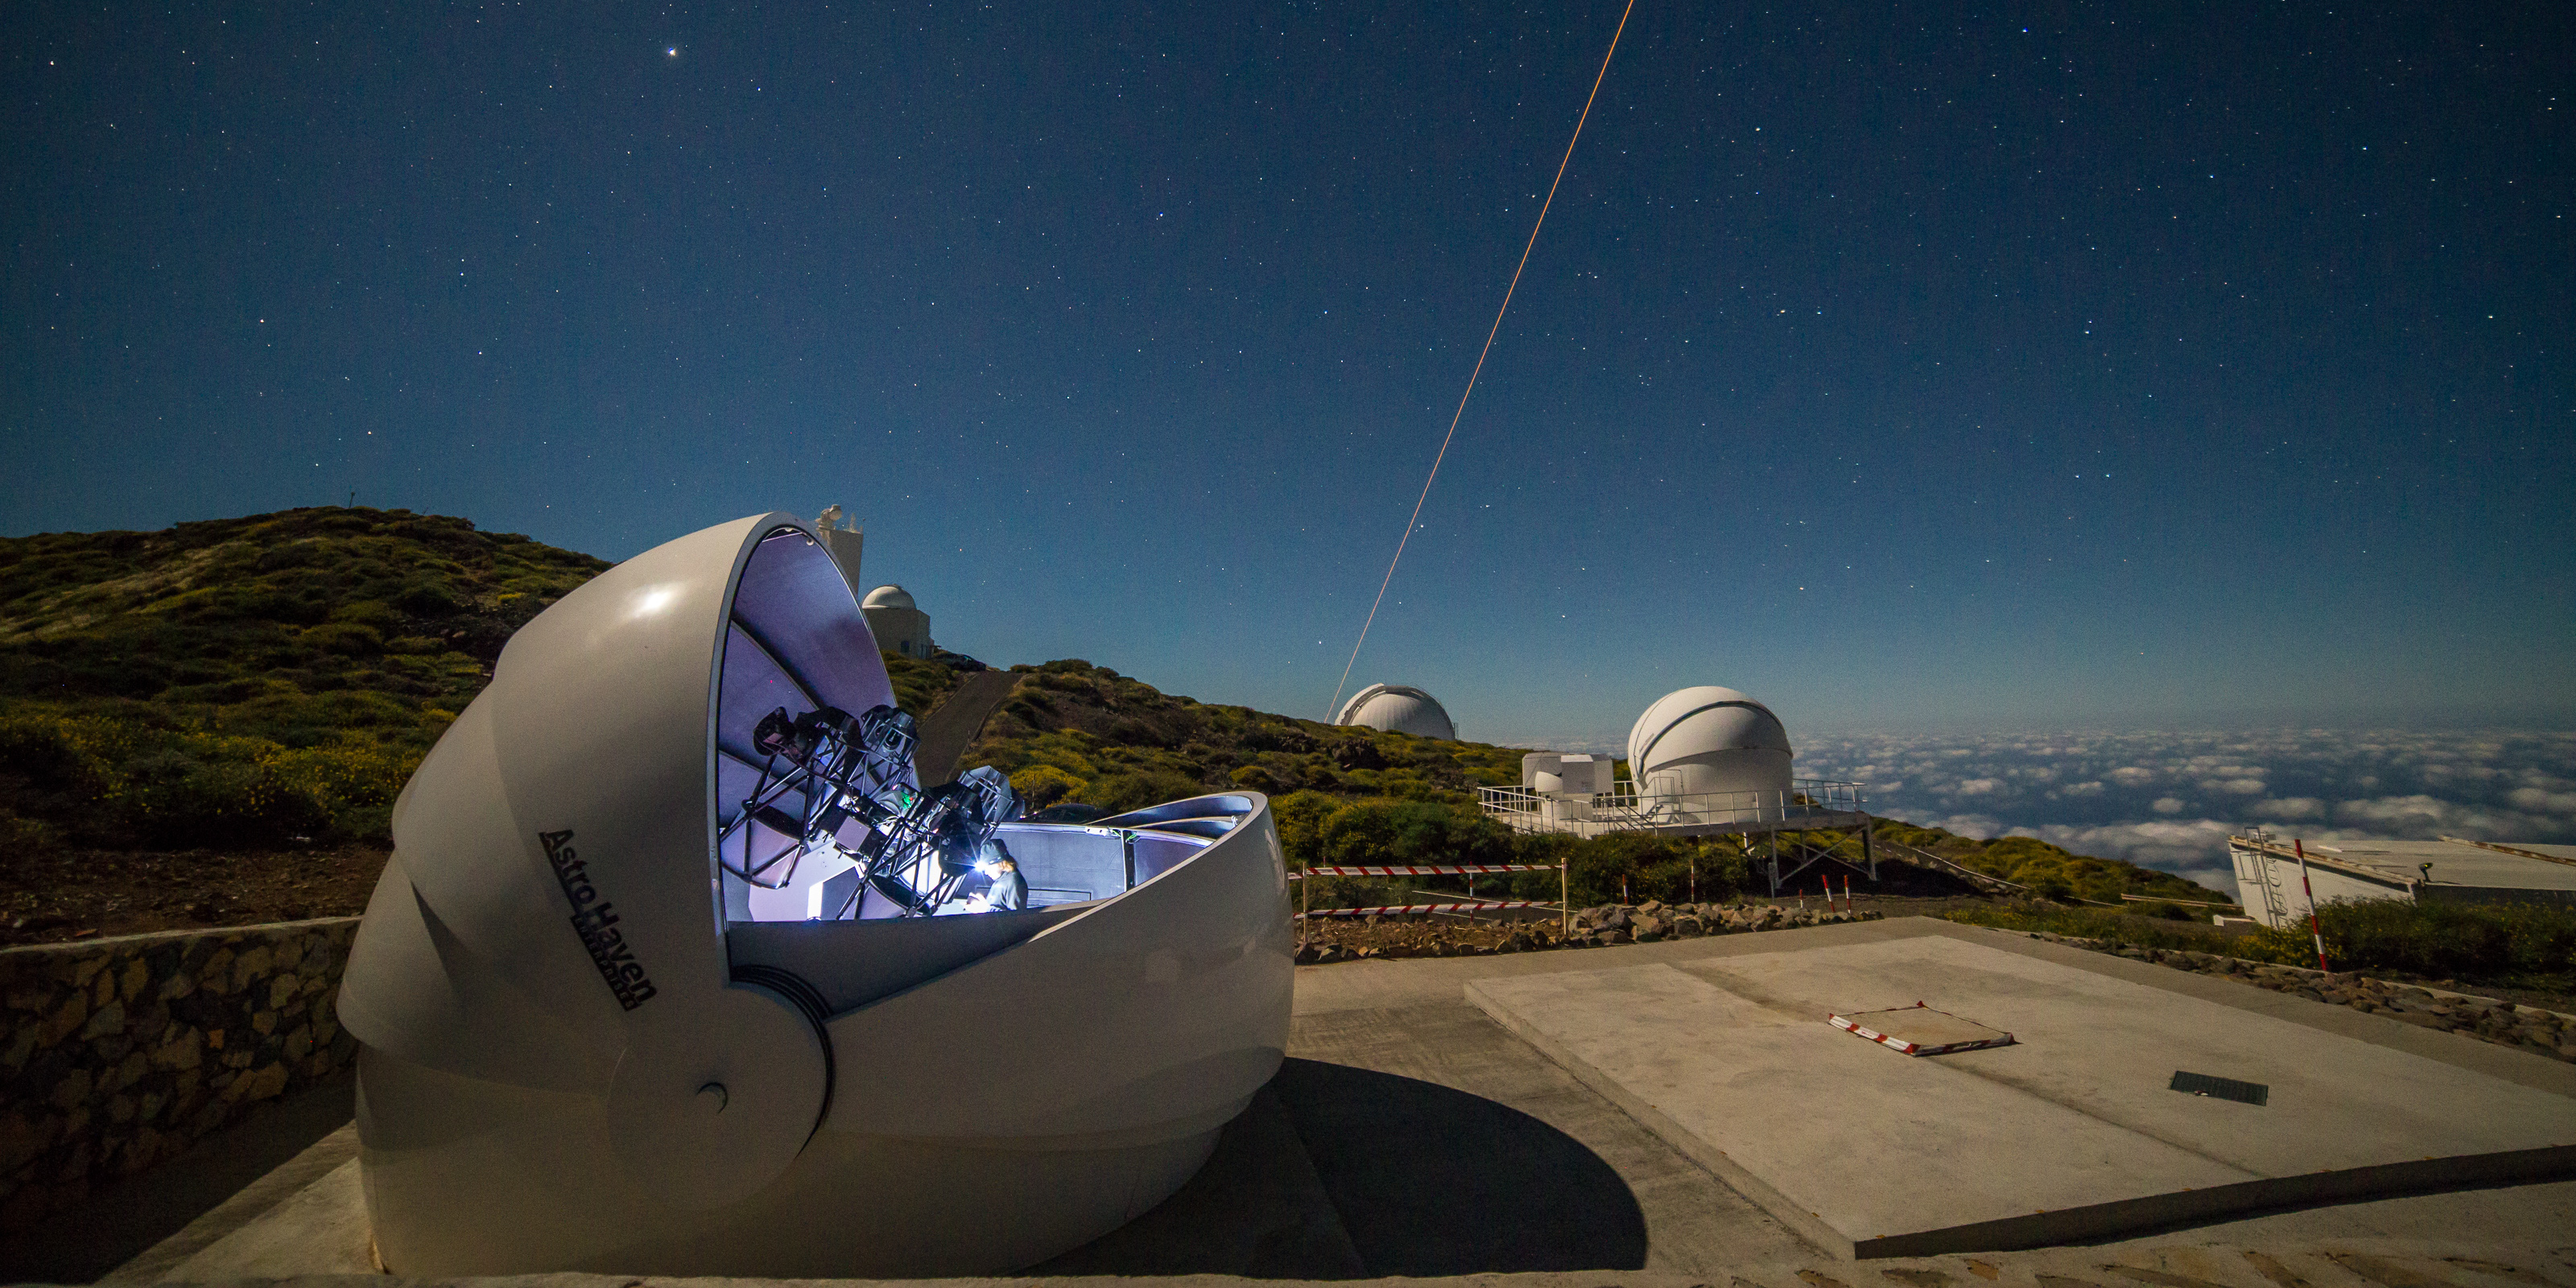
\includegraphics[width=\textwidth]{images/inauguration_photo.jpg}
    \end{center}
    \caption[Working in the GOTO dome prior to the inauguration in June 2017]{
        Working in the GOTO dome prior to the inauguration in June 2017. Photo taken looking west towards W1m and the WHT (with the orange ELT test laser visible). The empty platform on the right is where the second dome was installed later in the year.
    }\label{fig:inauguration}
\end{figure}

Unfortunately in the months after the inauguration problems began to surface with the hardware. The first problem was the failure of the declination motor encoder shortly after the inauguration. We were able to operate the telescope in a limited RA survey mode (described in \aref{sec:challenges}), however this greatly limited the capability of the telescope. There were also other problems with the guide mounts that hold the unit telescopes to the boom arm becoming lose, as well as the arms being too short so the telescopes could hit the mount. These issues meant that for the first few months of commissioning someone always needed to be present in the dome, so they could stop the mount moving if it was in danger of damaging itself. Once the O2 observing run ended there was less of a reason to be observing in this limited mode, so GOTO was shut down during the autumn until hardware upgrades could be installed at the start of November.

At the same time problems with the optical performance had become apparent, which were blamed on the mirror quality and issues with collimation. A program of sending each set of mirrors back to the factory one at a time was decided on, allowing GOTO to still operate with the remaining three. The worst performing telescope, UT3, had its mirrors taken out and returned in August. Once the telescope was reactivated in November the remaining three active unit telescopes were aligned to form a single 3$\times$1 footprint, shown in \aref{fig:3ut_footprint}. Counterweights were placed in the empty UT3 tube to allow the mount to still be balanced. GOTO operated in this mode for over a year, with the downtime from the gravitational wave detectors giving time to fully test the control software as well as develop the back-end image pipeline and classification systems (\todo{see intro}). The first set of mirrors were returned to the site in June 2018 and were placed into UT4, which was the second-worst performing. The old UT4 mirrors were sent back to the factory and GOTO continued to operate with three unit telescopes until February 2019. At this point, based on the imminent start of the third LIGO-Virgo observing run, it was decided to leave the other two mirrors and operate from then on in the designed 4-UT configuration shown in \aref{fig:4ut_footprint}.

One of the other problems found during commissioning was excessive scattered light entering the system, in particular light from the Moon entering the corrector lens. This was solved by adding covers around the telescope tubes, which prevented light from entering the corrector but made the system more susceptible to wind-shake (the reason that the tubes were designed as open in the first place). Ultimately the covers provided enough benefits, including protecting the mirrors from dust, that it is planned that future unit telescopes will have a closed tube design from the start.

\newpage

\begin{figure}[p]
    \begin{center}
        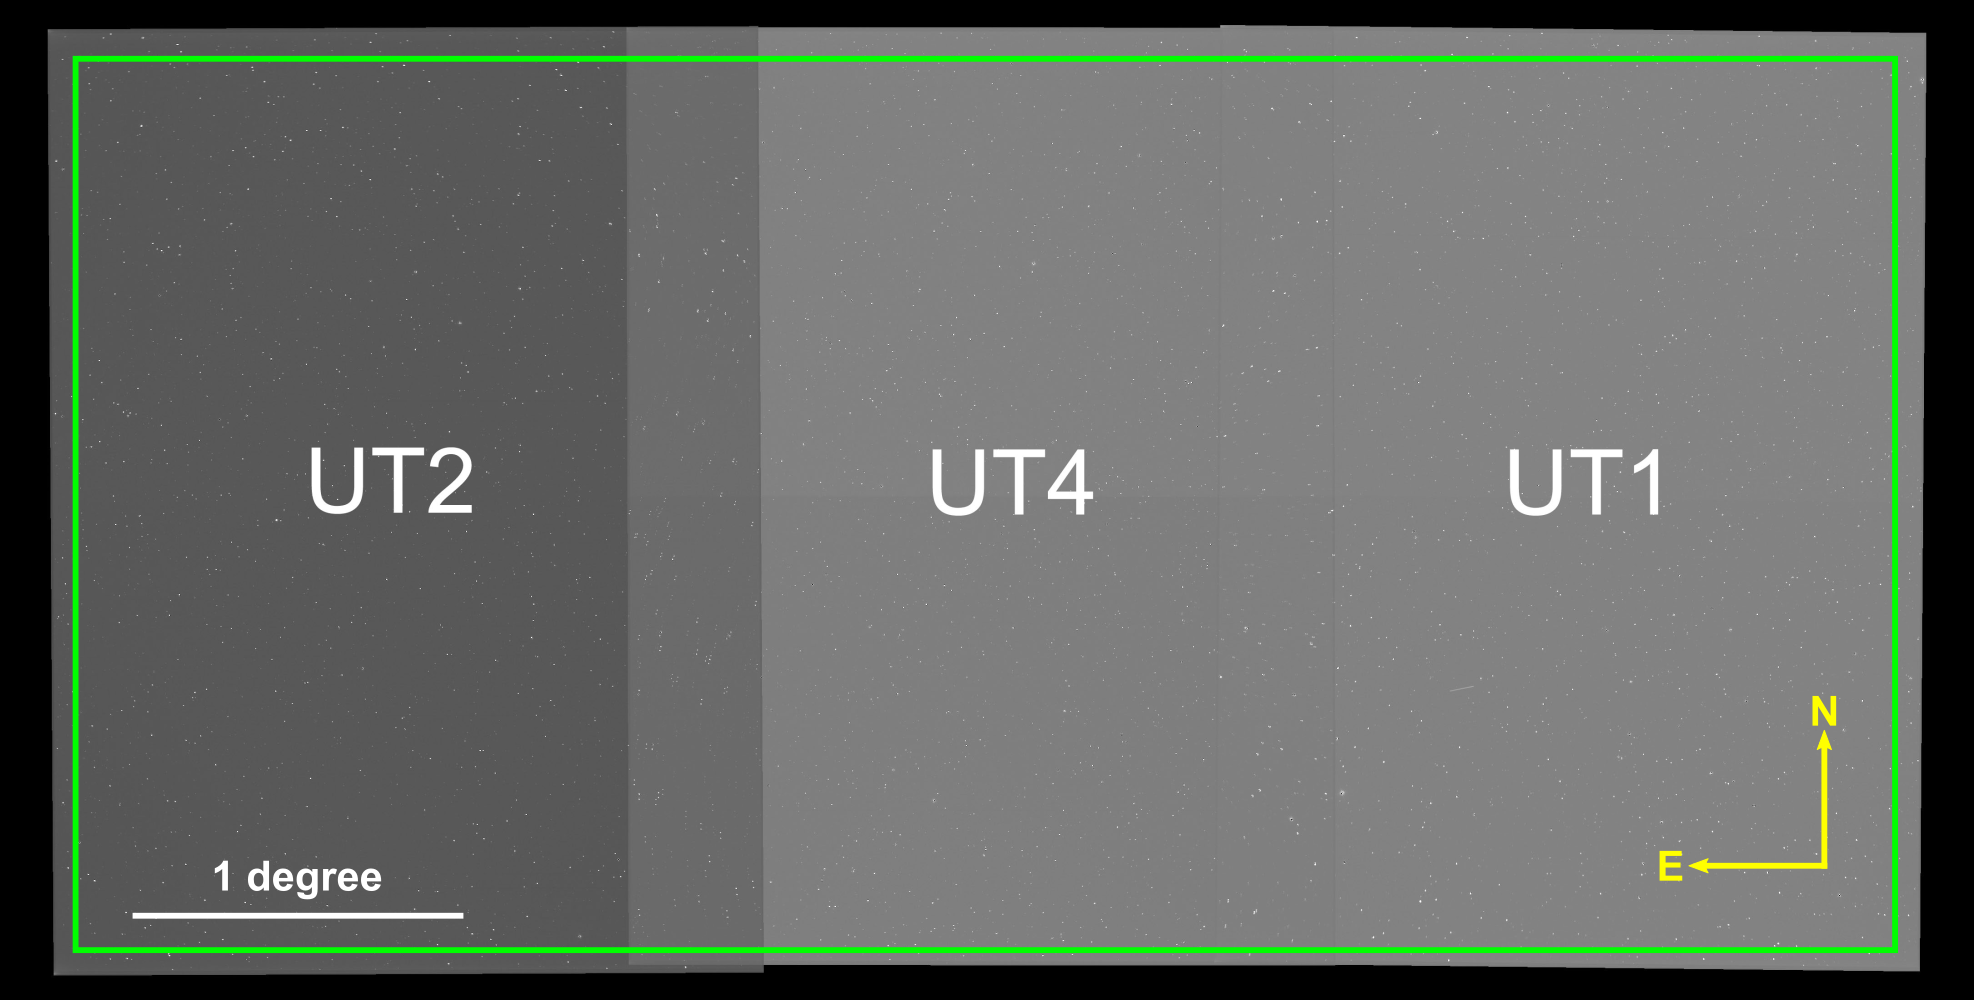
\includegraphics[width=0.7\textwidth]{images/footprint_1_box.png}
    \end{center}
    \caption[The previous 3-UT GOTO footprint]{
        The previous 3-UT GOTO footprint, used from August 2017 to February 2019. The initial $5.5 \times 2.6$ degree tile area is shown in \textcolorbf{Green}{green}. Note that a reasonable amount of space is left around the edge of the tile.
    }\label{fig:3ut_footprint}
\end{figure}

\begin{figure}[p]
    \begin{center}
        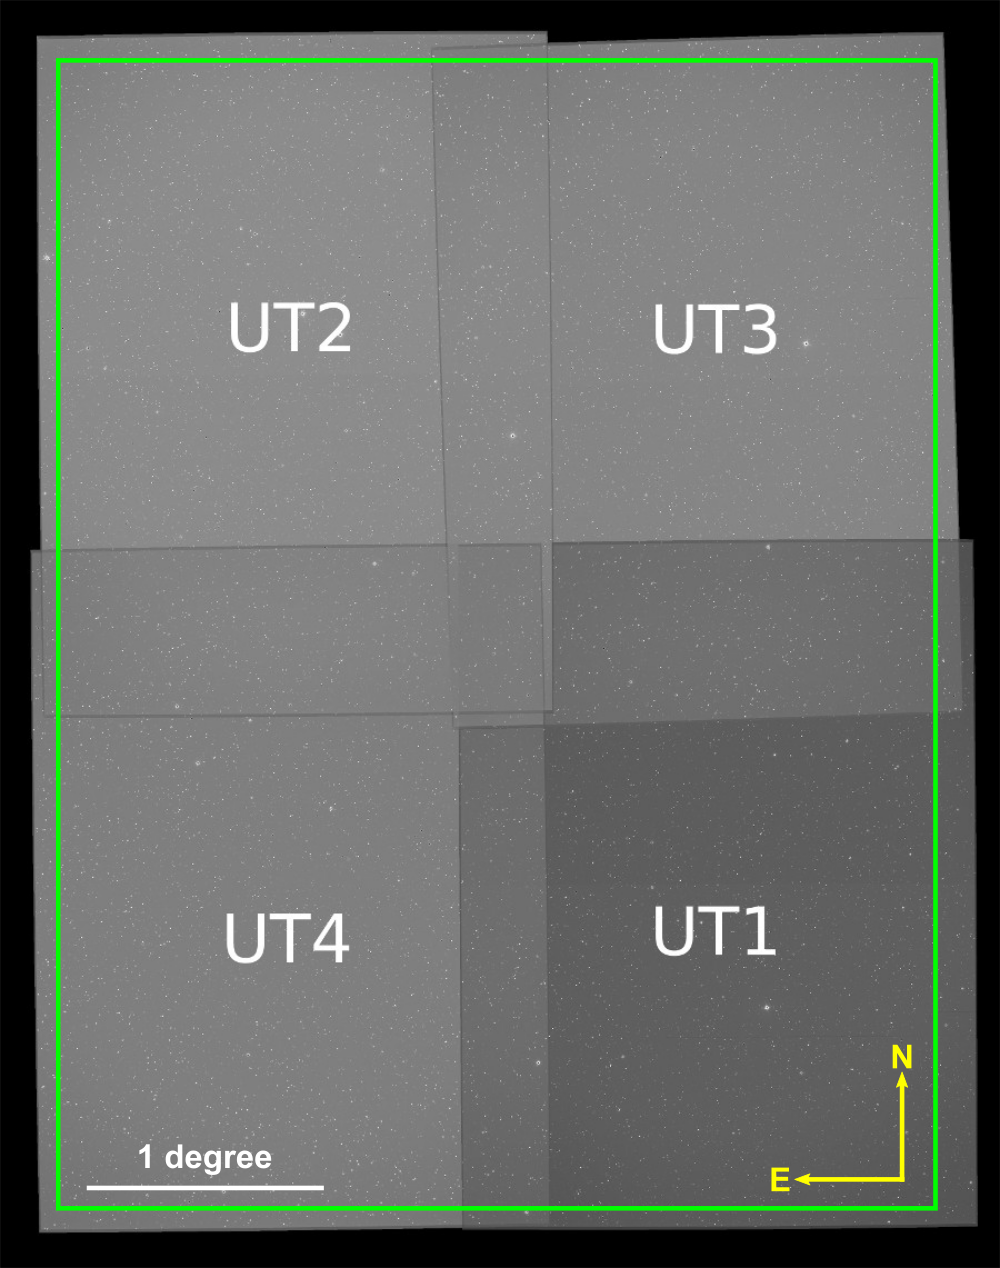
\includegraphics[width=0.6\textwidth]{images/footprint_2_box.png}
    \end{center}
    \caption[The current 4-UT GOTO footprint]{
        The current 4-UT GOTO footprint, in use from February 2019 onwards. The revised $3.7 \times 4.9$ degree tile area is shown in \textcolorbf{Green}{green}.
    }\label{fig:4ut_footprint}
\end{figure}

\clearpage

\begin{figure}[t]
    \begin{center}
        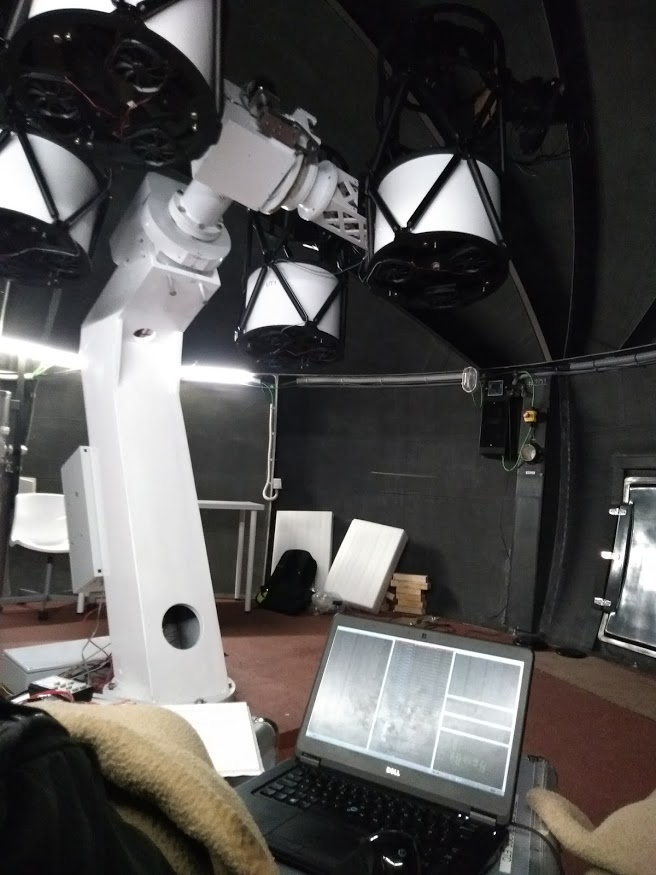
\includegraphics[width=0.4\textwidth]{images/commissioning_photo.jpg}
        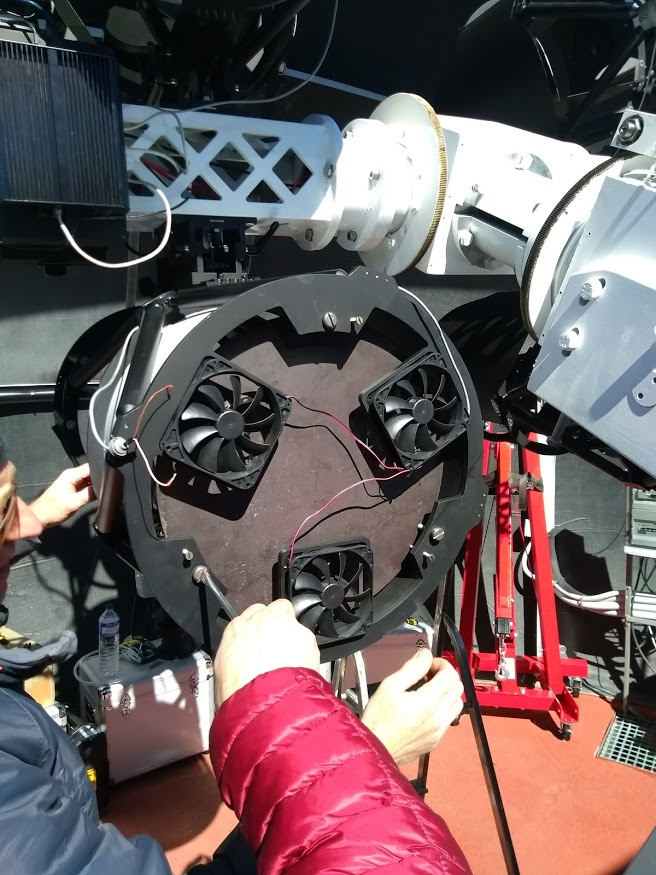
\includegraphics[width=0.4\textwidth]{images/commissioning_photo3.jpg}
    \end{center}
    \caption[Photos from GOTO commissioning]{
        Photos from GOTO commissioning.\\
        Left: Monitoring the telescope from inside the dome, November 2017.\\
        Right: Fitting the mirror counterweights in UT3, January 2018
    }\label{fig:commissioning}
\end{figure}

The secondary software commissioning period ran from the telescope being reactivated in November 2017 through to May 2018. During this time the telescope was typically running robotically each night, however there was always a member of the collaboration on site in order to supervise and monitor it in case of problems. Over that period the monitor moved from physically sitting in the dome, to sitting in the relative comfort of the neighbouring SuperWASP server room, until finally in the last few months being able to monitor from the observatory residencia or one of the other telescopes. I visited La Palma twice during this period, with the first trip in November 2017 covering the first week of the monitoring period immediately following the hardware upgrades. Other volunteers and students covered up until Christmas, then commissioning halted over the holiday period before I returned to the site in January for a three week visit. The first week overlapped with Kendall Ackley from Monash as well as a team from Sheffield, including Vik Dhillon and Stu Littlefair, who where there to work on the separate HiPERCAM instrument on the GTC.\@ During this period we replaced the counterweights, rebalanced the mount and realigned the unit telescopes, and I continued the software work with a major update to the observing database. During the second week I monitored the telescope alone from SuperWASP, and worked on upgrading the pilot so it was able to run automatically entirely with no human supervision. In the third week the HiPERCAM team returned and I continued to monitor the telescope, however a severe snowstorm stopped all observing and confined us to the residencia.

\begin{figure}[t]
    \begin{center}
        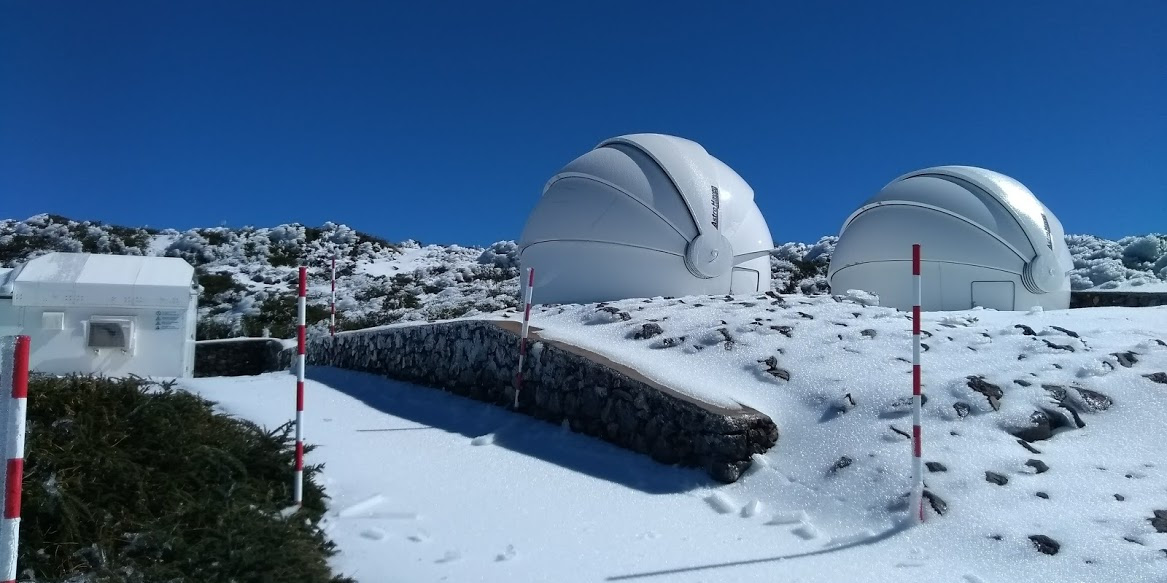
\includegraphics[width=\textwidth]{images/snow_photo.jpg}
    \end{center}
    \caption[The GOTO site shut down due to snow]{
        The GOTO site shut down due to snow, February 2018. Photo taken looking south-east, note the addition of the second dome compared to \aref{fig:inauguration}. SuperWASP is housed within the shed on the left.
    }\label{fig:snow}
\end{figure}

Due to the cold weather and ice build up GOTO was unable to open throughout all of February 2018, and the on-site monitoring only recommenced in the spring once the snow had melted. Monitors continued to be on site for several more months, in between hardware upgrade trips from Warwick, until eventually in May the software was deemed robust enough to allow GOTO to run unsupervised. The pilot output was still regularly monitored remotely, especially by the Australian team who had the benefit of a more convenient timezone. By the time the 4-UT system was recommissioned in February 2019 the pilot and hardware control systems had been fully tested and were operating reliably, and my focus had shifted to the alert follow-up systems in advance of O3.

\end{colsection}

% ~~~~~~~~~~~~~~~~~~~~

\newpage
\subsection{Additional dome systems}
\label{sec:arduino}
\begin{colsection}

GOTO uses a clamshell dome manufactured by Astrohaven, the same company that made the pt5m dome \citep{pt5m}. Based on experience with p5tm the there were several hardware systems which would be useful to add to the GOTO dome. In fact the entire pt5m dome control unit was replaced by a custom one designed and manufactured in Durham, however if possible we wanted to avoid such a drastic step. Several limitations of the stock dome are outlined below.
%
\begin{itemize}
    \item First, there was no easily-accessible emergency stop button to cut power to the dome in an emergency (e.g.\ something gets caught in the motors). This is a serious concern for pt5m as when the dome is open the shutters completely cover the access hatch, making it dangerous for anyone to be passing through the hatch when the dome is moving. Therefore one of the additions to pt5m was an emergency stop button within arms reach of the hatch entrance. As the GOTO dome is taller the hatch is still mostly uncovered when the dome is open, however installing an emergency stop button was still a priority.
    \item In a similar health and safety concern, by default the dome does not come with a siren to sound when it opens or closes. This is an important safety feature when operating a robotic observatory, as the dome will be operated entirely through software and it is important to warn anyone on site several seconds before it is about to move. When members of the GOTO team are on-site the robotic systems can be disabled entirely by going into engineering mode (see \aref{sec:mode}), however it is still important to make sure there is no chance of the dome moving without prior warning. In addition, the GOTO site on La Palma is completely publicly accessible, and it is not unknown for tourists or hikers, or other astronomers, to be around the dome when it is unsupervised.
    \item By default the dome \glsfirst{plc} only provides limited information about the status of the dome shutters. As described in \aref{sec:dome}, the \gls{plc} only returns a single status byte in response to a query. This is not enough to distinguish whether the dome is fully or only partially open, and if one side is moving the status of the other side is unknown. It is possible to determine the current status by saving the previous status within the dome daemon, but having constant on/off switches would be more reliable.
    \item The dome comes with two in-built magnetic sensors on each side, which should detect when the shutters are either fully closed or fully open. However these have been know to be unreliable and tricky to align. In some cases the switches failed to trigger when the shutter reached its open limit, leading to the dome continuing to drive the belts and the shutter embedding itself into the ground. Therefore having secondary, independent sensors was a priority to ensure this did not happen.
    \item One final proposed addition was a quick-close button, which acts as a simple and direct way to communicate with the dome daemon. The motivation is a practical one: in the case that the weather turns bad and the telescope is exposed, assuming the automatic monitoring systems fail and we can't connect to close it remotely, it is a lot easier to direct someone on site to access the dome and press the prominent ``close'' button than direct them to log on to the in-dome computer, open a terminal and type \code{dome close}. In turn during the commissioning phase, when the software was still being tested and someone has to be on duty on-site all night, it is easiest if they have a single, simple button for them to press if they feel any rain. One requirement was that this button could not be easily confused with the emergency stop button (i.e.\ it should not be coloured red), as instead of stopping the dome this button will prompt it to move.
\end{itemize}
%
Adding an emergency stop button to the dome was fairly simple. As shown in \aref{fig:estop_plc} there was enough slack on the power cable for the PLC to install a prominent red button on the wall of the dome. When the button is pressed the power to the PLC is cut, which will prevent commands being sent to the dome motors and therefore stop them moving.

\begin{figure}[p]
    \begin{center}
        \includegraphics[width=0.8\textwidth]{images/estop_photo.jpg}
    \end{center}
    \caption[The dome PLC and emergency stop button]{
        The dome \glsfirst{plc} and emergency stop button. The green cable comes directly from the dome power supply at the top, passes through the button unit and into the PLC at the bottom.
    }\label{fig:estop_plc}
\end{figure}

\newpage

\begin{figure}[t]
    \begin{center}
        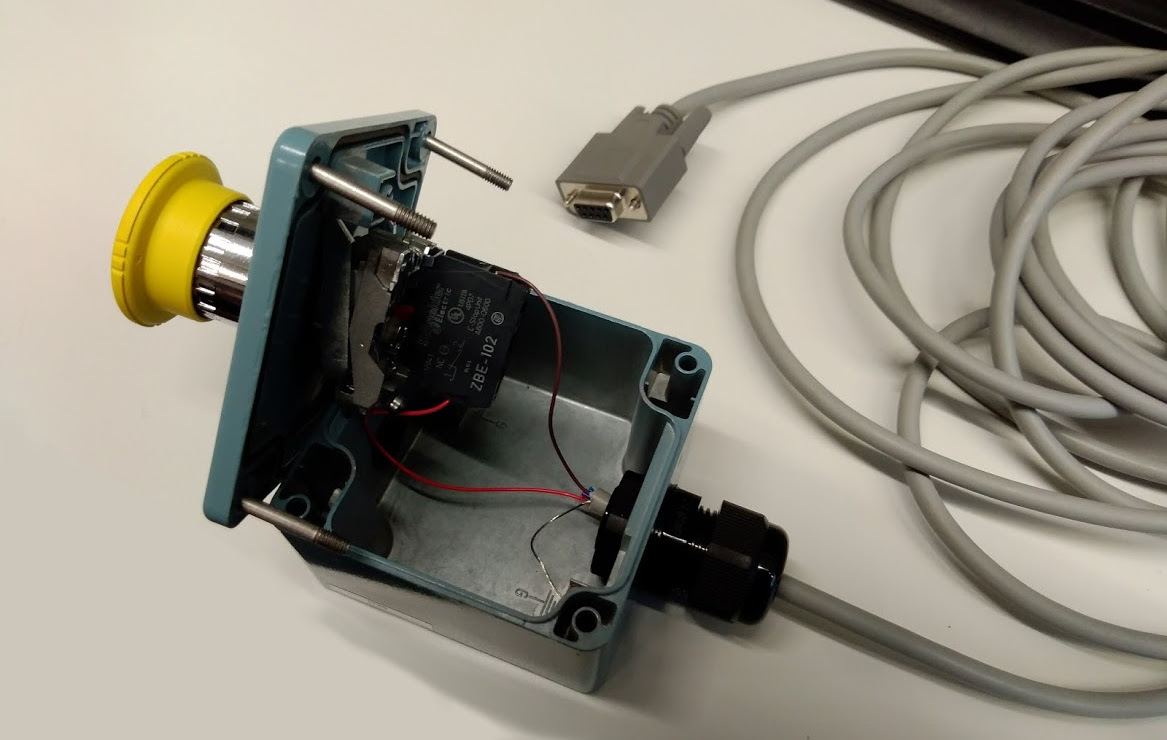
\includegraphics[width=0.9\textwidth]{images/button_photo.jpg}
    \end{center}
    \caption[Building the quick-close button]{
        Building the quick-close button in the lab in Sheffield. The transmit wire is coloured brown and the receive wire is coloured pink, these are attached to the button NC pins.
    }\label{fig:quickclose_button}
\end{figure}

Creating a quick-close button involved attaching a ``normally closed'' (NC) push button in serial between the transmit and receive wires of an RS 232 serial cable. By doing this a simple feedback loop can be set up within the dome daemon, by sending a test signal out through the serial connection and listening for it to be returned to the same port. If after three tries the signal does not return then the button has been pressed, and the dome daemon triggers a lockdown (see \aref{sec:dome}). By using a locking push button the loop will remain broken, and the dome closed, until the button is released. As shown in \aref{fig:quickclose_button} a bright yellow button was chosen, this was clearly labelled and attached to the wall of the dome near the computer rack as shown in \aref{fig:arduino_button_dome}.

Adding a siren and more sensors to the dome required an additional system to power, monitor and (for the siren) activate them. This was done using a small Arduino Uno microcontroller\footnote{\url{https://www.arduino.cc/}} running a simple HTML server, which reports the status of the switches and can be queried in order to activate the siren. The circuit design for this system is shown in \aref{fig:arduino_circuit}. In order to power the siren from the Arduino a bipolar MOSFET (metal-oxide-semiconductor field-effect transistor) was used to connect to one of the the board input/output pins, with a large enough resistor to prevent the voltage from frying the board. The Arduino and siren were set within a weatherproof case, with output connectors for the dome switches as well as for power and an ethernet connection. Photos of the box during construction are shown in \aref{fig:arduino_wip}, and its installation in the dome is shown in \aref{fig:arduino_installed} and \aref{fig:arduino_button_dome}.

Four additional switches were added into the dome, each connected to a port on the Arduino through the connectors on the bottom of the box. Two Honeywell limit switches were attached to the sides of the dome, set to be triggered when the dome was fully open. An additional magnetic proximity switch was added to the two inner-most shutters which will trigger when the dome is fully closed. Finally a second magnetic switch was added to the dome hatch. Each of these are shown in \aref{fig:dome_switches}.

\begin{figure}[t]
    \begin{center}
        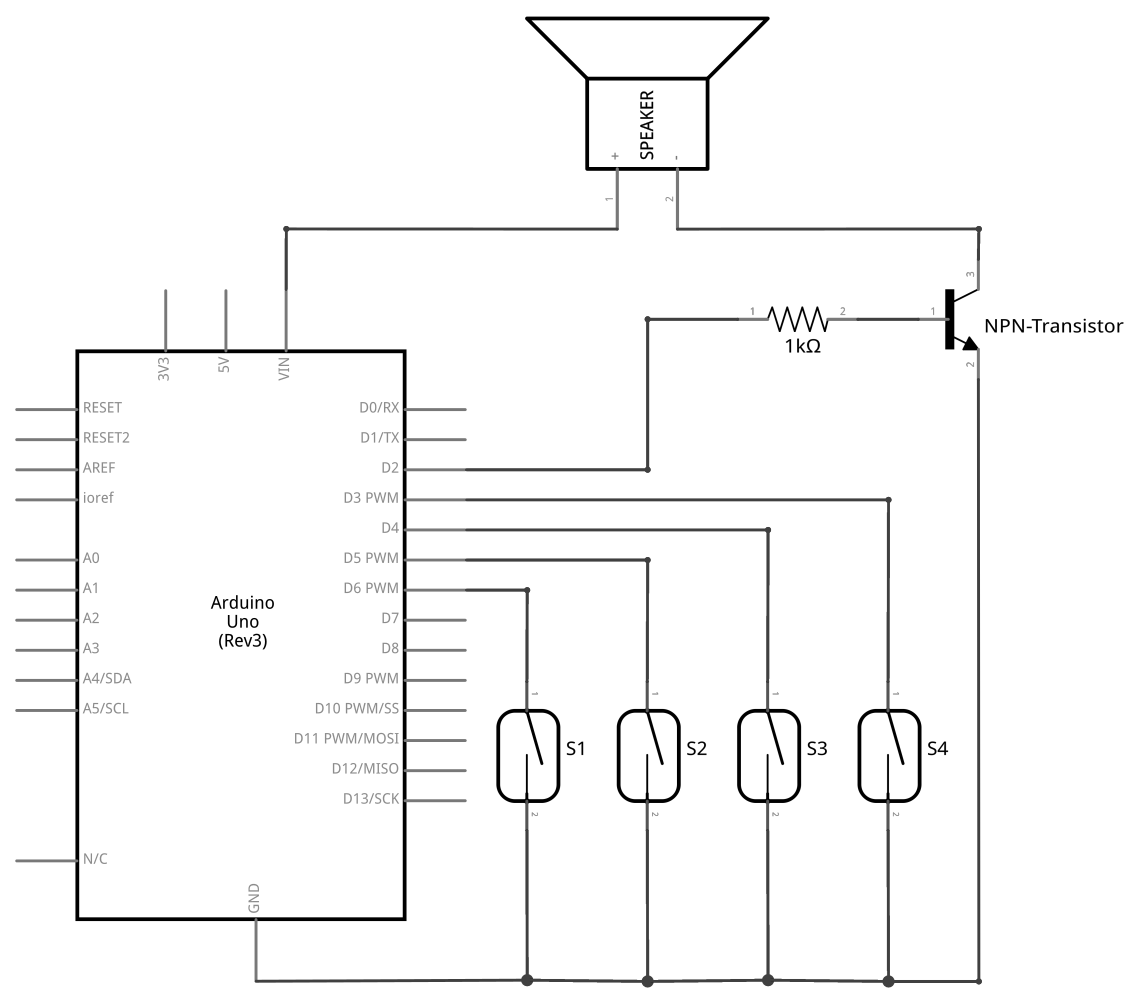
\includegraphics[width=0.75\textwidth]{images/arduino.png}
    \end{center}
    \caption[Circuit design for the Arduino box]{
        Circuit design for the Arduino box.
    }\label{fig:arduino_circuit}
\end{figure}

\begin{figure}[p]
    \begin{center}
        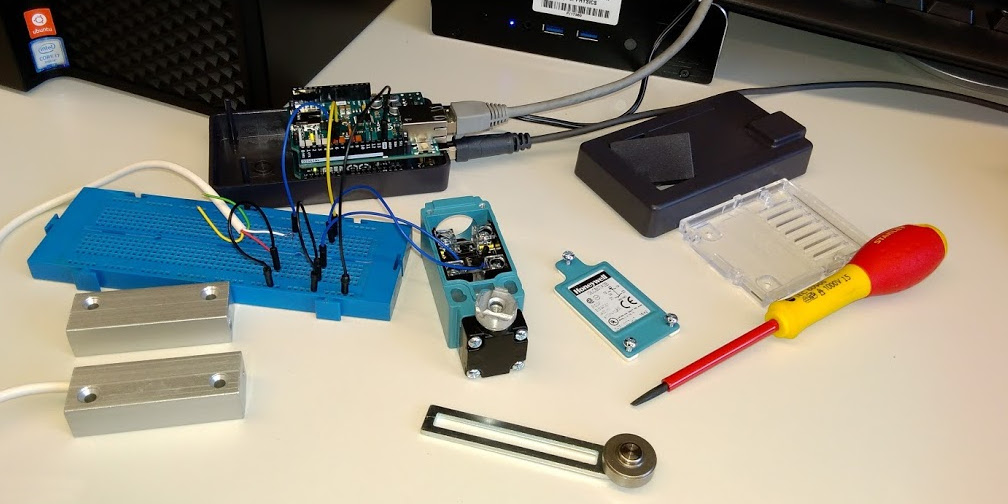
\includegraphics[width=\textwidth]{images/arduino_photo.jpg}
        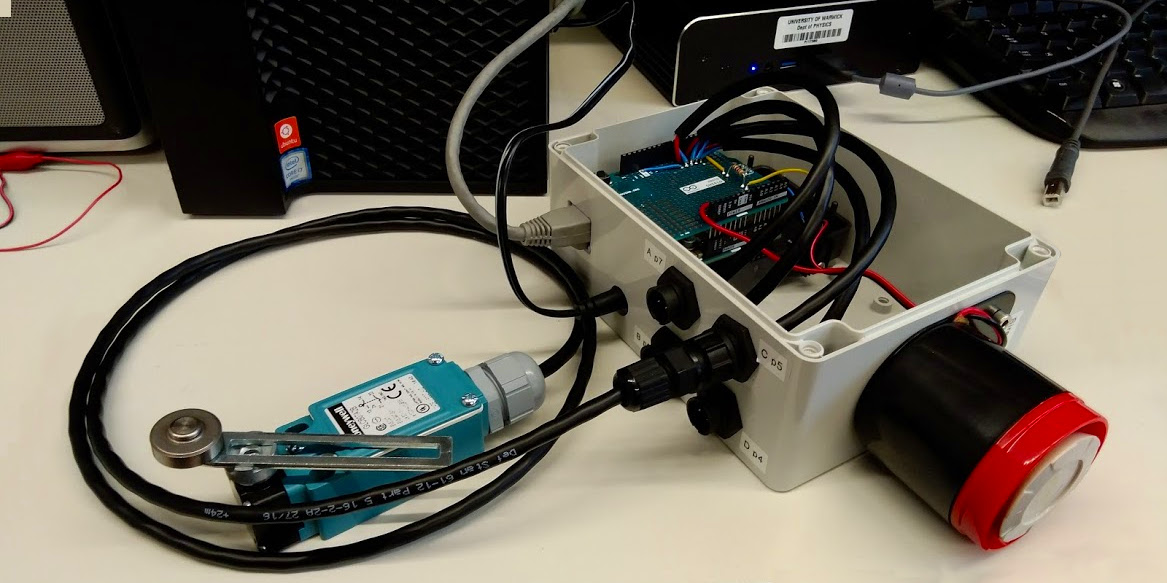
\includegraphics[width=\textwidth]{images/box_photo.jpg}
    \end{center}
    \caption[Building the dome Arduino box]{
        Building the dome Arduino box in the lab in Sheffield.\\
        Top: Testing the circuit design with the Arduino (circuit board in the back) and two of the dome switches: a magnetic security switch (grey blocks on the left) and a Honeywell limit switch (cyan unit in the centre, with the cover and arm detached).\\
        Bottom: The completed box, showing the Arduino, power and ethernet cables, siren, and one of the four switches.
    }\label{fig:arduino_wip}
\end{figure}

\newpage

\begin{figure}[p]
    \begin{center}
        \includegraphics[width=0.75\textwidth]{images/box_installed_photo.jpg}
    \end{center}
    \caption[The Arduino box installed in the GOTO dome]{
        The Arduino box installed in the GOTO dome during my first trip to La Palma in March 2017. This photo was taken before the cover and cables were attached.
    }\label{fig:arduino_installed}
\end{figure}

\begin{figure}[p]
    \begin{center}
        \includegraphics[width=0.75\textwidth]{images/box_installed_photo2.jpg}
    \end{center}
    \caption[The Arduino box and quick-close button in the GOTO dome]{
        The Arduino box and yellow quick-close button in the GOTO dome, attached to the southern pillar under the dome drive. The cables run to the computer rack which is just off to the left of the photo.
    }\label{fig:arduino_button_dome}
\end{figure}

\newpage

\begin{figure}[p]
    \begin{center}
        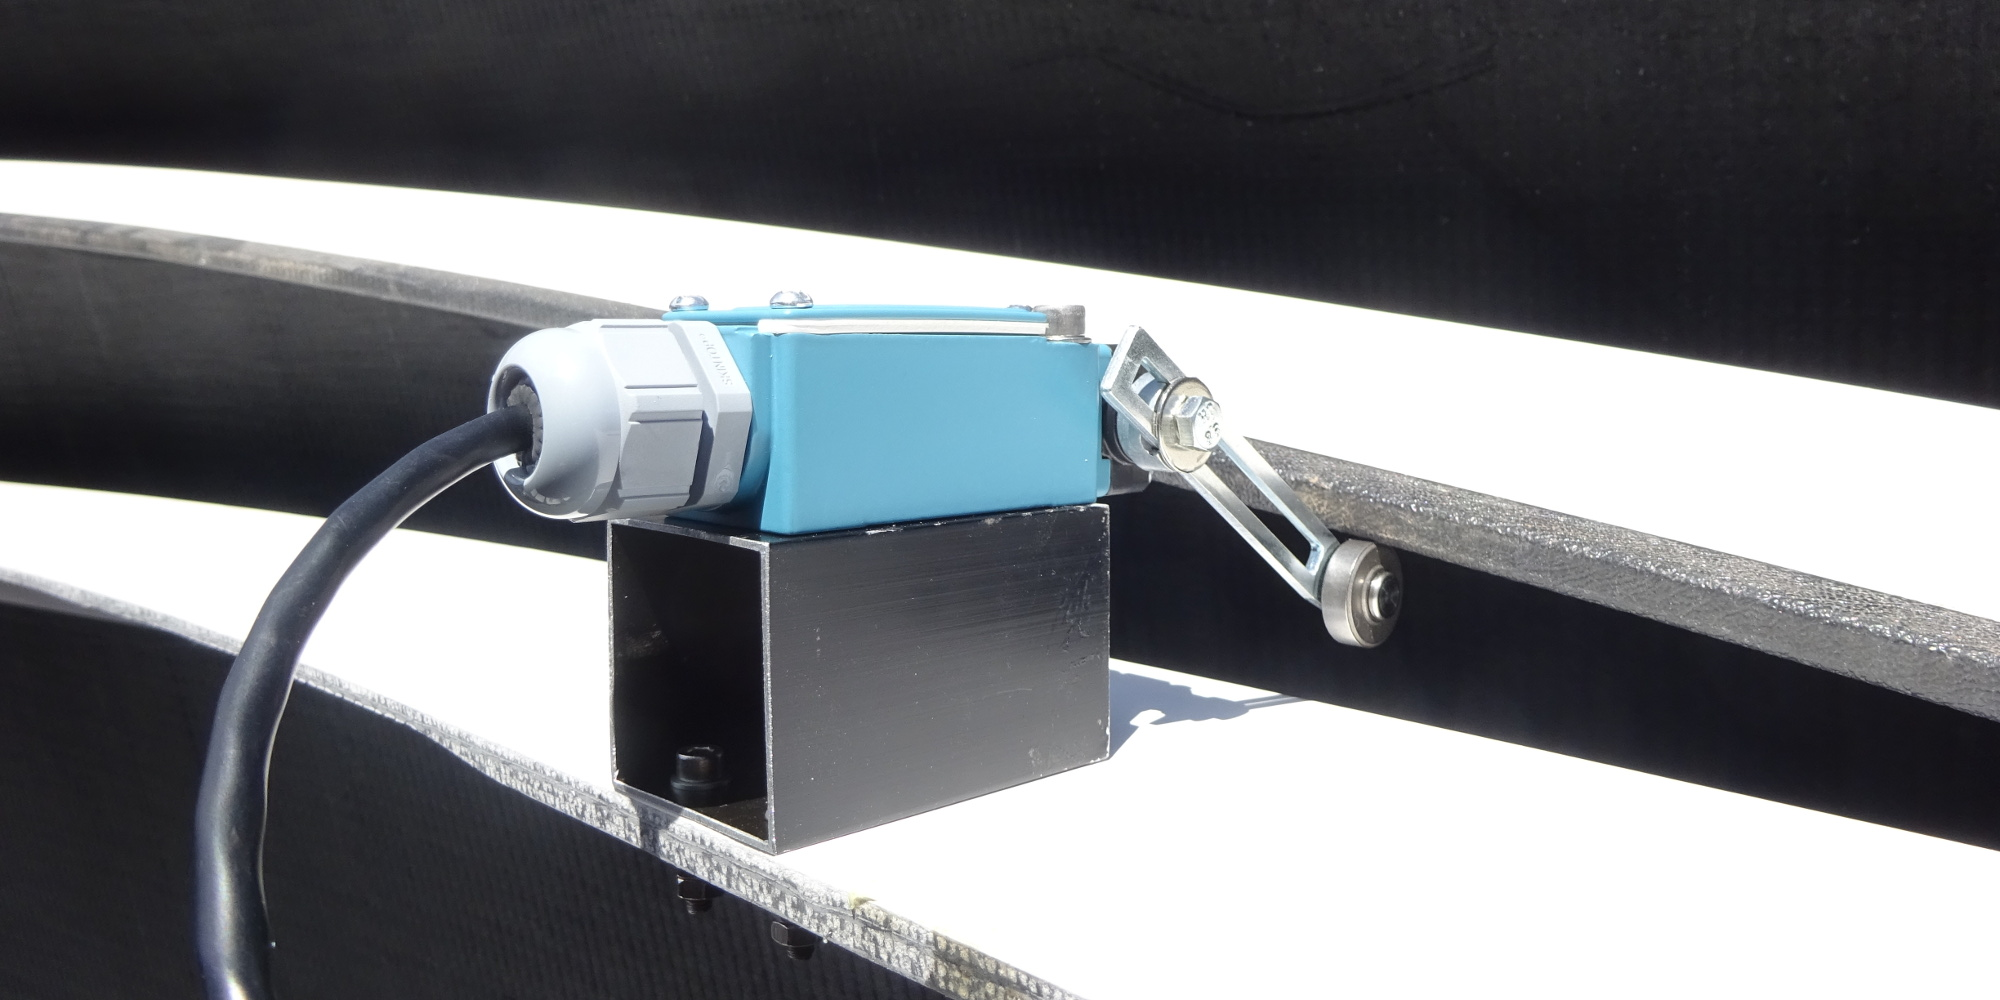
\includegraphics[width=0.8\textwidth]{images/dome_sensor_1.jpg}
        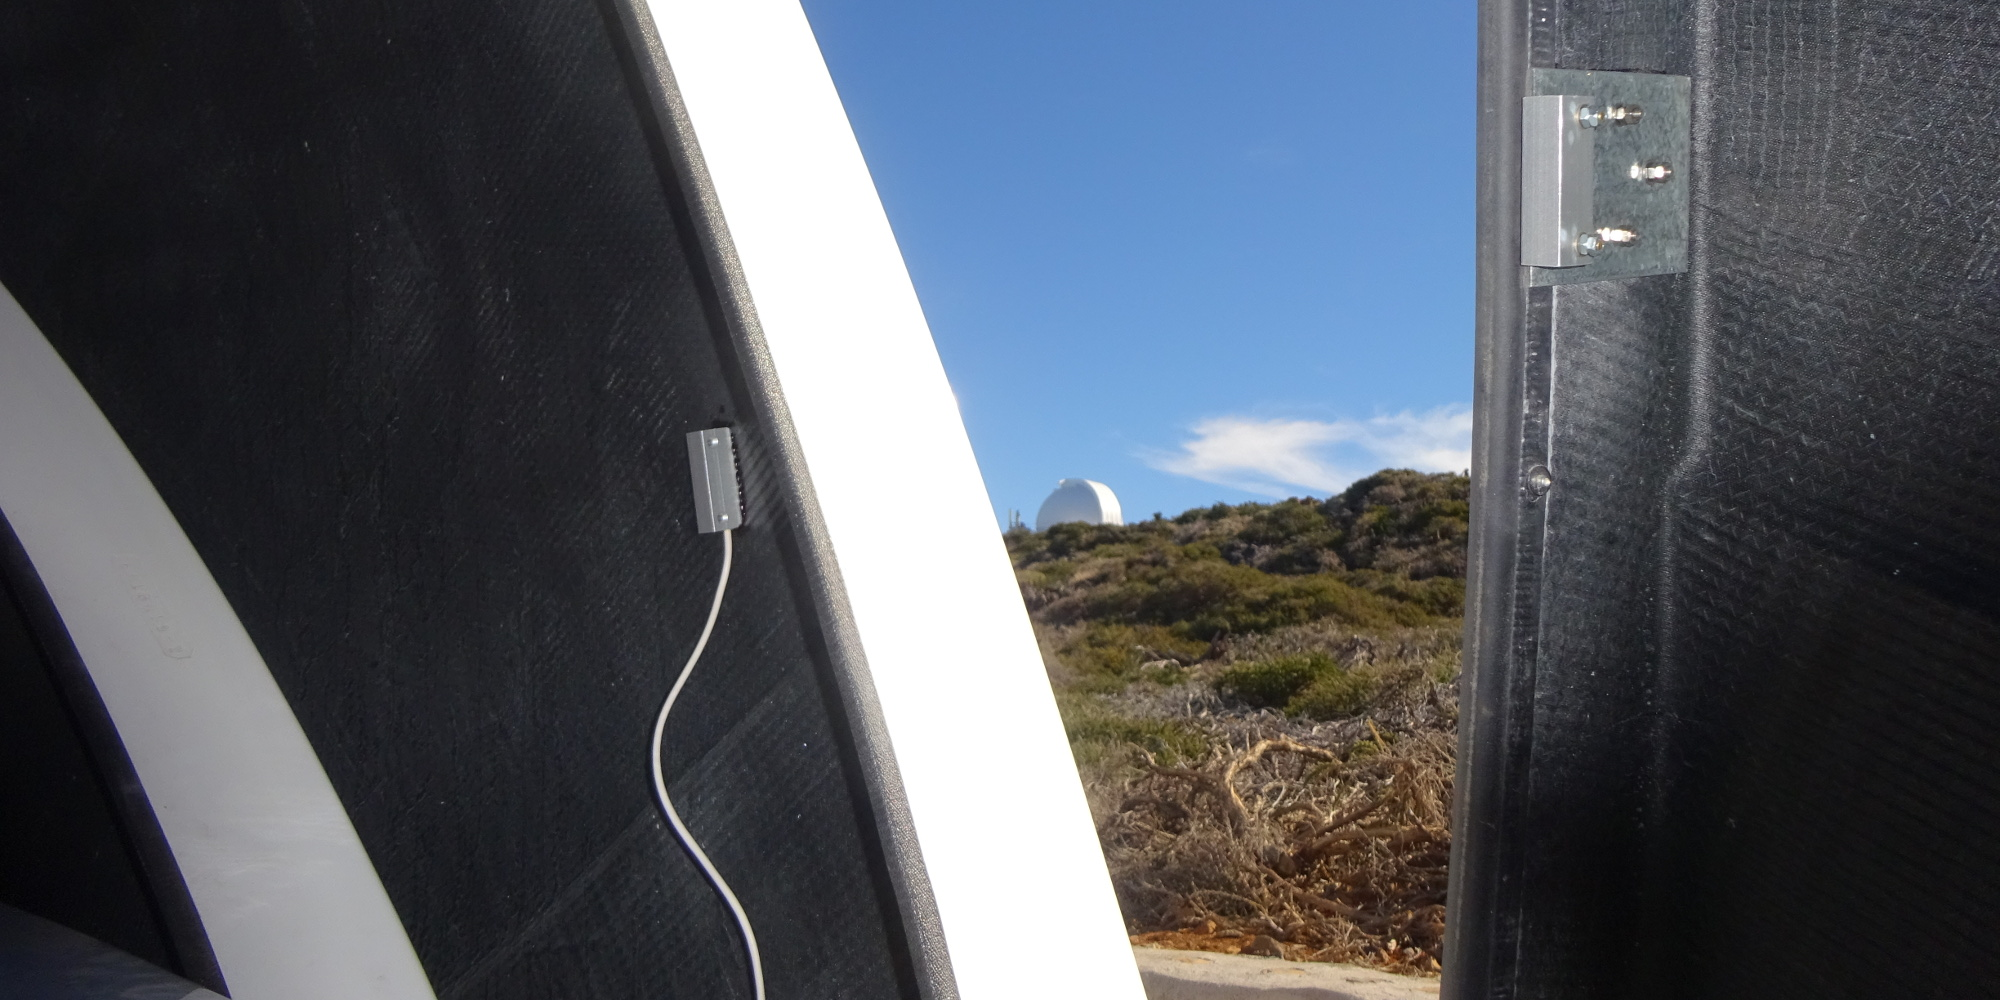
\includegraphics[width=0.8\textwidth]{images/dome_sensor_2.jpg}
        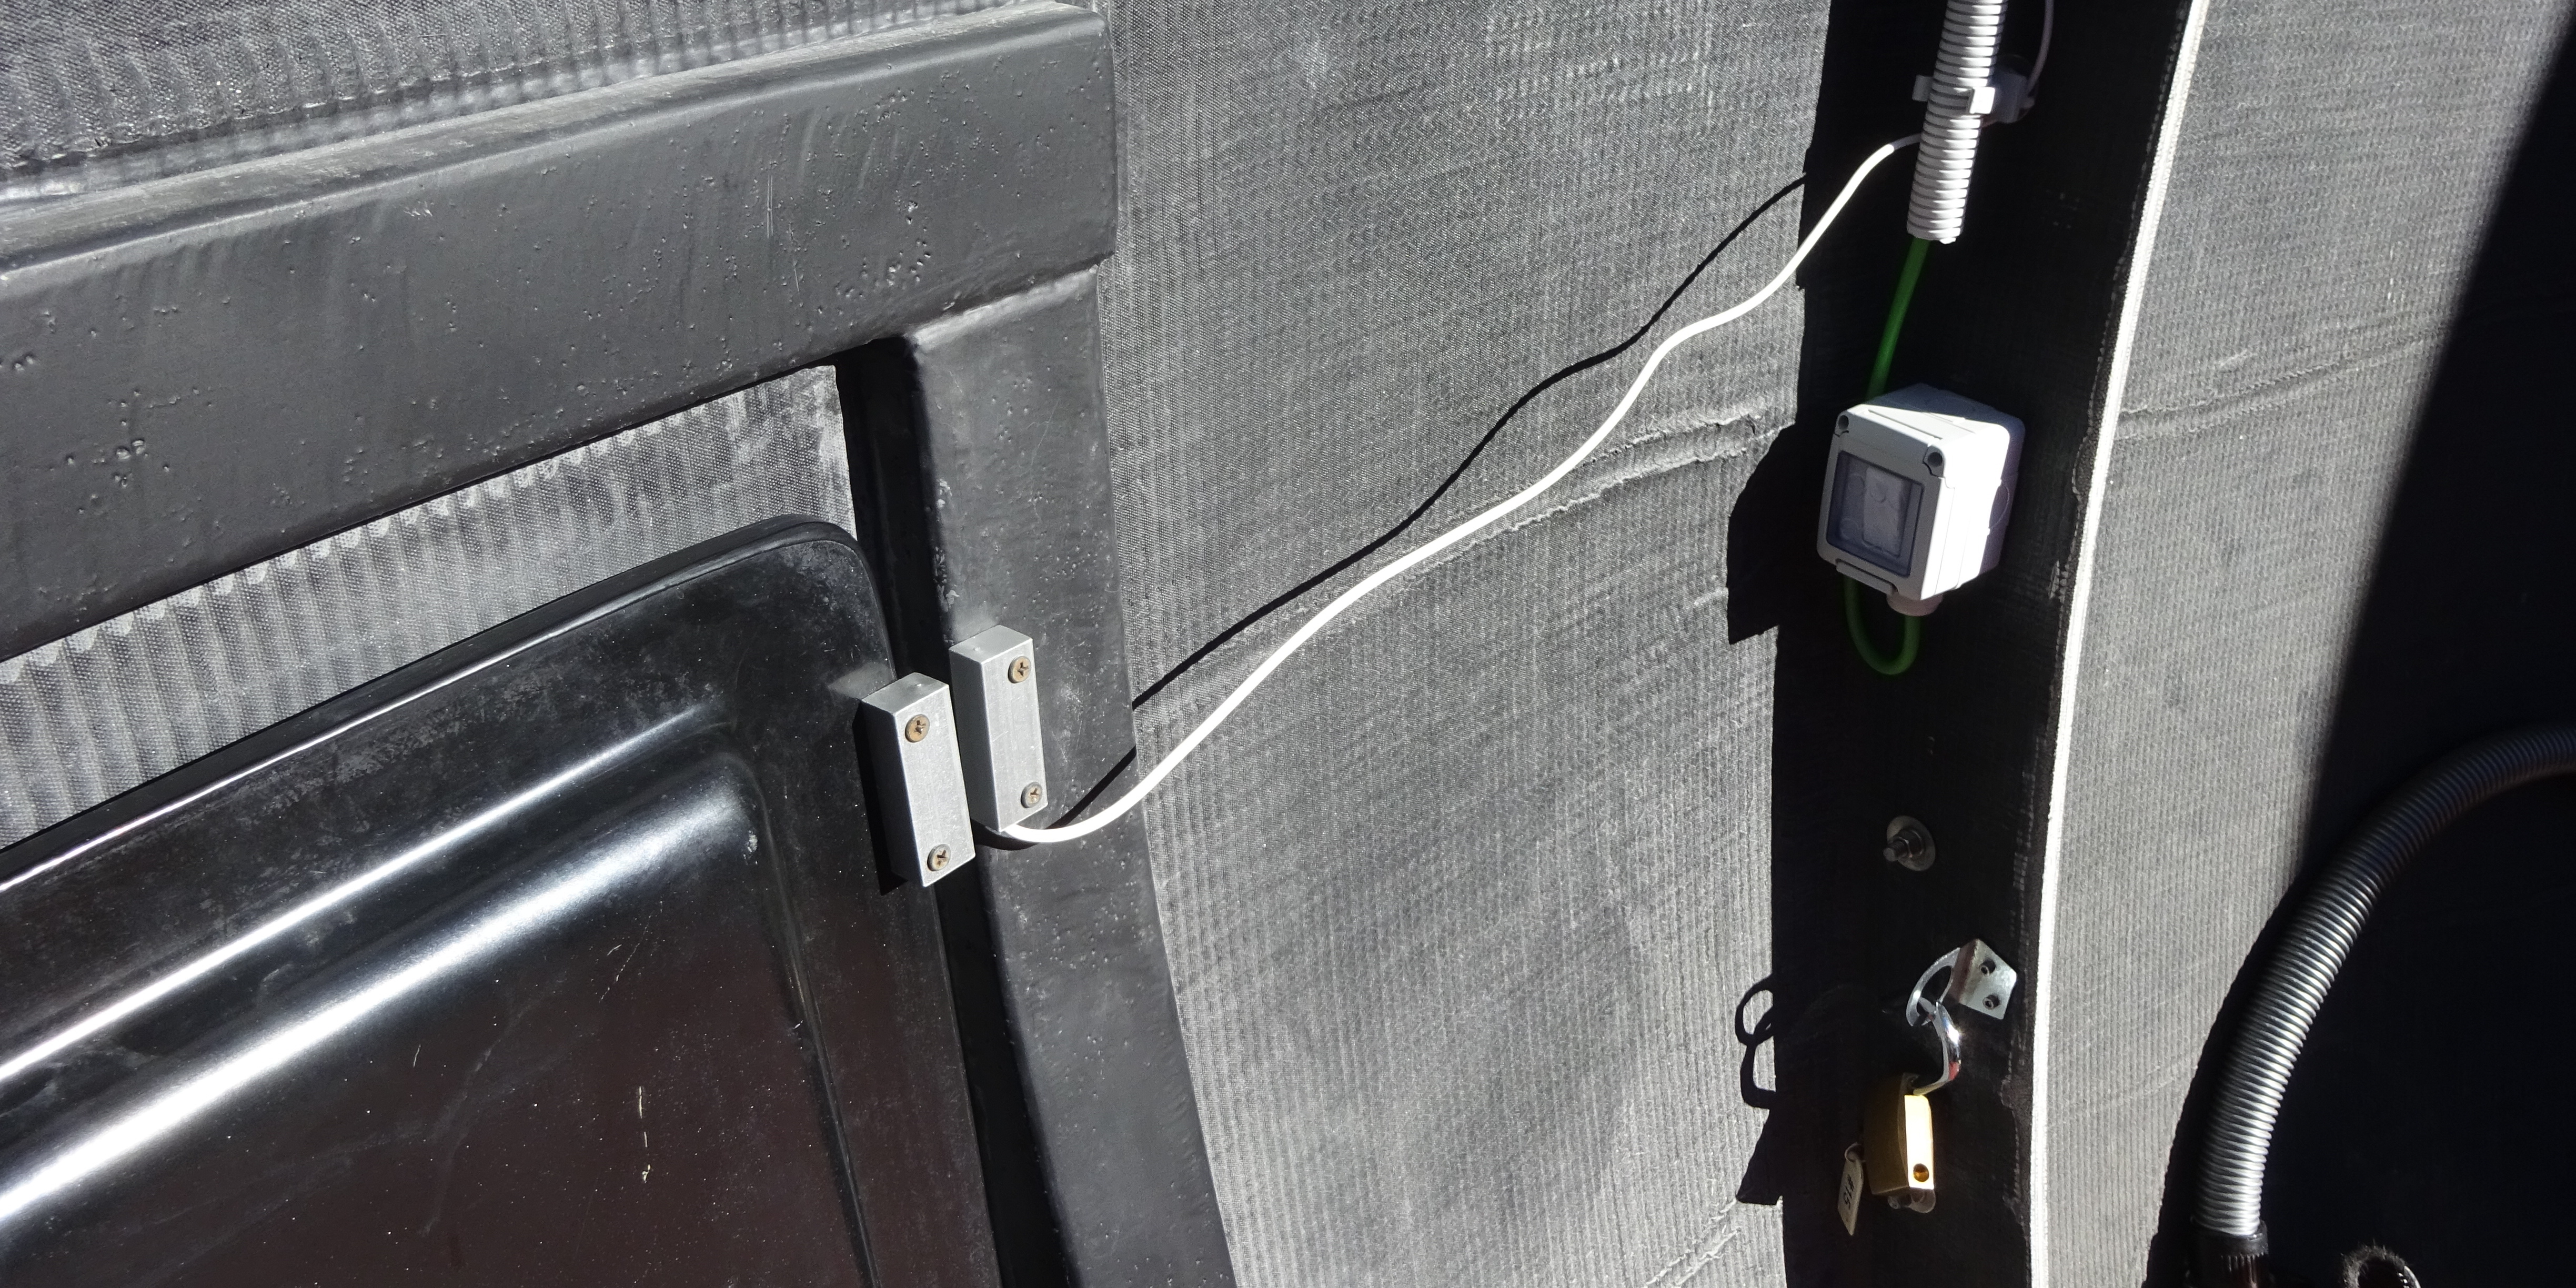
\includegraphics[width=0.8\textwidth]{images/dome_sensor_3.jpg}
    \end{center}
    \caption[Additional sensors added to the dome]{
        Additional sensors added to the dome during the March 2017 trip:\\
        Top: One of the two limit switches added to detect when the dome is fully open.\\
        Middle: The magnetic switch added to detect when the dome is fully closed.\\
        Bottom: The magnetic switch added to the dome hatch to detect if it is open or closed.
    }\label{fig:dome_switches}
\end{figure}

\clearpage

Using a combination of these new switches and the PLC output is is possible for the dome daemon to build up a complete status of the dome. The software implementation of this is described in \aref{sec:dome}. Having a sensor on the hatch also allowed it to be added as a conditions flag as described in \aref{sec:conditions_flags}, meaning the pilot will stop and report if the hatch is open when in robotic mode. As of yet the hatch flag or in-dome buttons have not been needed in an emergency, however they are important as an insurance policy just in case. It is anticipated that the same work will need to be done in the second GOTO dome when it is commissioned. Comments have also been passed on to Astrohaven to suggest they could include some of the features in their own stock hardware, for example a built-in siren that could be optionally sounded whenever the dome is moving.

One further addition to the GOTO dome should be mentioned: the ``heartbeat'' monitor designed and installed by Paul Chote at Warwick. As described in \aref{sec:dome}, in the event that the dome daemon crashes or the control NUC itself fails for whatever reason the dome would be left vulnerable --- especially if it was already open. As a backup Paul created his own Arduino system that connects to the dome PLC and will send it commands to close in the event that it does not receive a regular signal from the dome daemon. This system was installed into the GOTO dome in April 2018, along with the other Warwick telescopes on the site, and was one of the final stages required before GOTO could safely leave the commissioning phase and not require an on-site monitor. As a similar new addition to the domes Paul used some of the ideas from the system outlined here, for example integrating a siren into the W1m unit. When the second GOTO dome is commissioned we will consider if the two systems could be merged.

\end{colsection}

% ~~~~~~~~~~~~~~~~~~~~

\end{colsection}

% ########################################

\newpage
\section{Developing the software}
\label{sec:software_commissioning}
\begin{colsection}

% ~~~~~~~~~~~~~~~~~~~~

\begin{colsection}

While the GOTO hardware was being commissioned the G-TeCS control software was also being developed. There were several important parts of the software that could not reasonably be developed without access to the actual telescope, notably developing observing routines such as taking flat fields or autofocusing.

Note this section focuses on the software side of commissioning, and does not include pure hardware issues such as with the mount drive, mirrors or guidemounts outlined in \aref{tab:timeline}. These were dealt with by the core GOTO hardware team at Warwick, and although I spent plenty of time on La Palma balancing the mount, adjusting mirror positions and aligning unit telescopes it had limited impact on the control software development.

\end{colsection}

% ~~~~~~~~~~~~~~~~~~~~

\subsection{Taking flat fields}
\label{sec:flats}
\begin{colsection}

\todo{WIP}
\citep{flats}

\end{colsection}

% ~~~~~~~~~~~~~~~~~~~~
\newpage
\subsection{Focusing the telescopes}
\label{sec:autofocus}
\begin{colsection}

\todo{WIP}
\citep{autofocus}

\end{colsection}

% ~~~~~~~~~~~~~~~~~~~~
\newpage
\subsection{Creating a pointing model}
\label{sec:pointxp}
\begin{colsection}

\begin{figure}[t]
    \begin{center}
        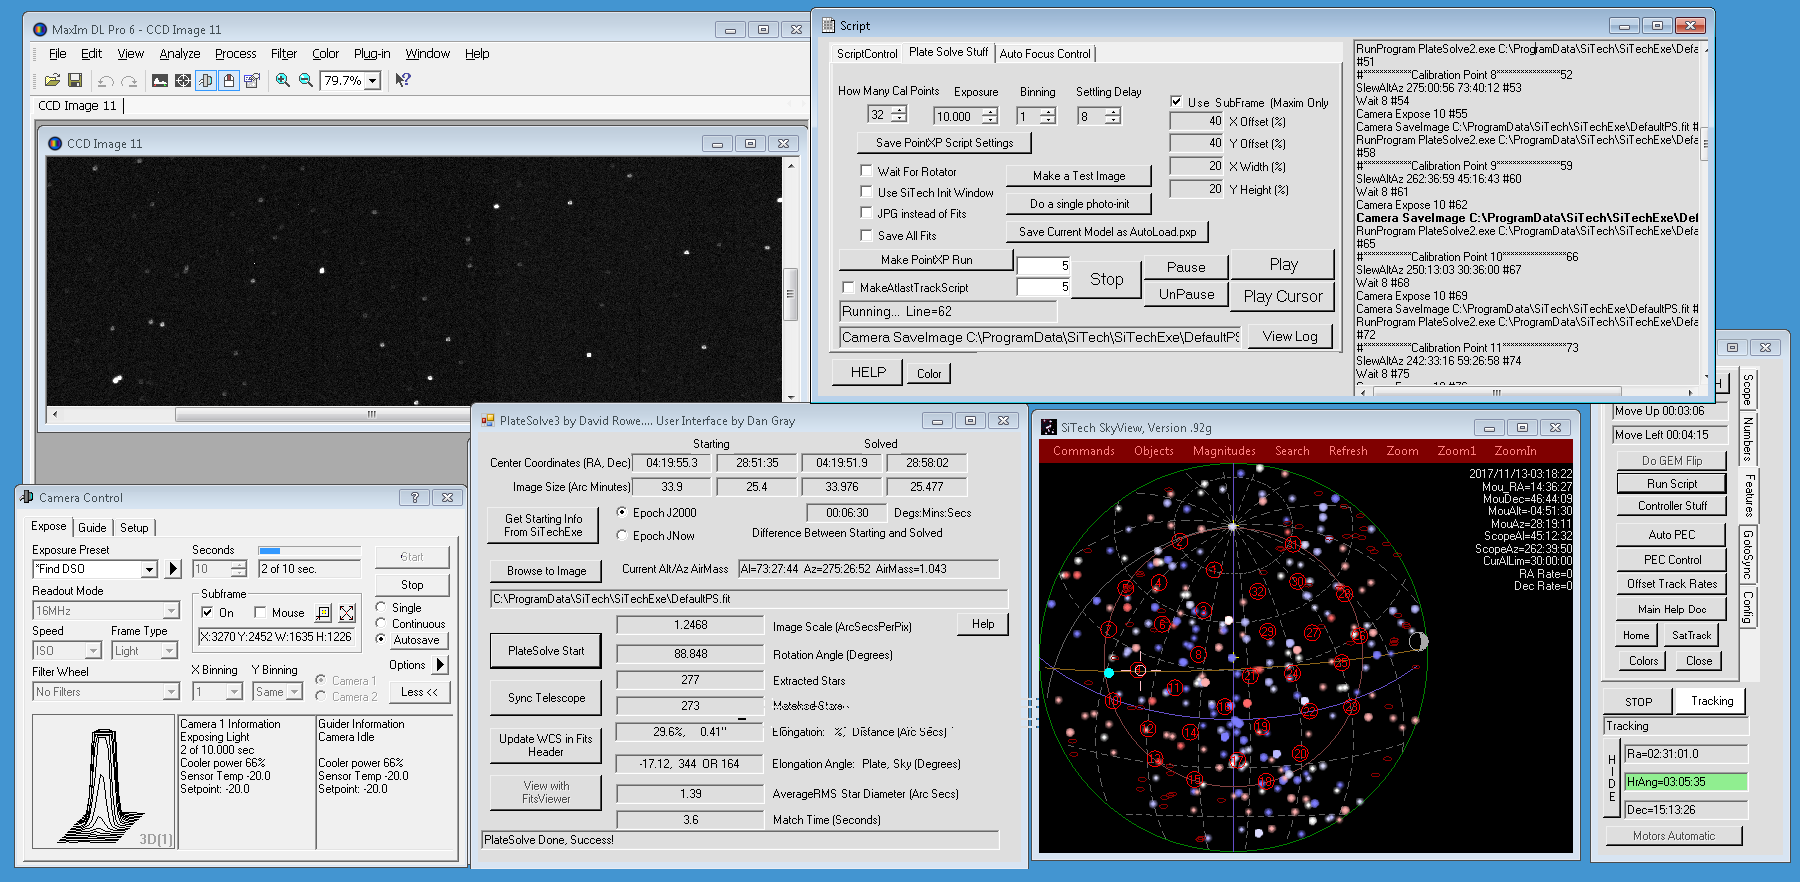
\includegraphics[width=\textwidth]{images/pointing_model.png}
    \end{center}
    \caption[Creating a pointing model using PointXP]{
        Creating a pointing model using PointXP.\@
    }\label{fig:pointing_model}
\end{figure}

Mount balancing and pointing model with PointXP

\end{colsection}

% ~~~~~~~~~~~~~~~~~~~~

\newpage
\subsection{Other commissioning challenges}
\label{sec:challenges}
\begin{colsection}

In this section I outline a few of the other hardware-related challenges that the software had to overcome. This is not an exhaustive list, and several of the software-only changes were already discussed in the relevant section in \aref{sec:hardware_control} (for example changing the mount control from requiring a Windows interface).

% ---------
\subsubsection{Filter wheel serial numbers}

One of the hardware issues that was identified early on concerned identifying the filter wheels when they were connected to the interface NUCs. The usual way to connect to specific hardware units through the \pkg{fli-api} package is to search the connected USB devices for their unique FLI serial numbers (for example the serial numbers of the GOTO cameras given in \aref{tab:cameras}). However the initial set of CFW9--5 filter wheels delivered to us by FLI did not have serial numbers defined. As on the mount two filter wheels were connected to each interface NUC this problem made it impossible to send individual commands to each through the software.

A solution was eventually found using the \proglang{Python} \pkg{pyudev} module, which uses the Linux \code{udev} device manager to identify devices using the \code{/dev/} name, and therefore create a pseudo-serial number based on which port each device was connected to. Using this method it is possible to tell apart filter wheels as long as you knew which physical USB port each was plugged into. This is not an ideal solution, but as long as the USBs remain connected it is not an issue even if the NUCs are rebooted.

% ---------
\subsubsection{Downloading images from the cameras}

One of the more complicated parts of the camera control software within \pkg{fli-api} is reading images from the FLI cameras. Once an exposure has finished counts from the chip are read out and stored in a buffer on the camera, where they can be downloaded by USB.\@ A last-minute change lead to the GOTO cameras using new, larger detectors than originally designed for the cameras, which lead to there not being enough space in the camera buffer to store a full-frame image. This was discovered when corrupted images such as the one shown in \aref{fig:cam_readout} were being produced; the regions in the lower third of the image are just duplicates of the data in the upper third meaning the original data in that section was lost.

\begin{figure}[t]
    \begin{center}
        
\includegraphics[width=0.7\textwidth]{images/cam_readout.png}
    \end{center}
    \caption[A corrupted image which was not read out fast enough]{
        An example of a corrupted image from one of the MicroLine cameras which was not read out fast enough.
    }\label{fig:cam_readout}
\end{figure}

The cameras return a \code{DataReady} status once the exposure has finished and the data is reading out, however when installing G-TeCS on site it was clear that the camera daemon was not able to reliably start downloading the data from the cameras quick enough to clear space in the internal buffer. The solution was to add an internal image queue within \code{fli-api}, which would immediately begin downloading from the cameras as soon as they reported the exposure was finished. This meant the camera data was stored within the memory on the interface NUCs, and then the camera daemon queried the \code{fli} interfaces (see \aref{sec:fli}) to download the images across the network.

This solution did run into a few problems with a feature of the Python programming language called the global interpreter lock (GIL), which prevents multiple threads accessing the same Python object at once (the exact workings of the GIL are out of scope for this thesis). In short this prevented reading out the cameras to the internal queue in parallel, which added extra delay time. Luckily the \pkg{fli-api} module was not written in standard Python (technically CPython) but in Cython, which interfaces between the FLI API code written in C and the rest of the system written in Python. Cython contains a GIL to maintain compatibility with CPython, however it is not required and can be disabled. Doing this allowed the cameras to be read out in parallel as intended.

% ---------
\subsubsection{Dec axis encoder failure}

Just a few weeks after the inauguration the mount declination axis encoder failed, preventing any automated slewing in the declination axis (the telescope could still be moved manually with the hand-pad). Of the two axes to fail this was by far the better one, had the RA axis failed instead then the telescope would not be able to track and images could not be taken. Instead the telescope could still take images, and commissioning the optics and the control software could therefore continue.

However when Stu and I visited in July 2017 we wanted to test the automated pilot, and the SiTech control software was not able to cope with the disabled dec axis. When sent a command to slew to a position it would move to the closest correct position in RA, however it would never register reaching the target and therefore would not start tracking. Instead a workaround was coded into the mount daemon, a separate thread which would monitor the RA position and stop moving when the target RA coordinates were reached regardless of the declination coordinates. Some other small changes were needed in the pilot and startup/shutdown scripts, as the mount was unable to officially park for the same reason. When these were in place GOTO was able to observe `normally', and with a limited set of targets added to the observing database the telescope could carry out a survey in a limited declination band of the sky.

Had an important gravitational wave target come through during this period the on-site monitor would have had to move the telescope to the correct declination and then manually carry out observations --- thankfully this was not needed and once O2 ended GOTO was shut down until the motors could be replaced.

% ---------
\subsubsection{Dome movement}

The Astrohaven clamshell dome is driven by internal belts attached to the dome shutters. It is important when moving the dome to not put undue stress on these belts, as should one of them dislodge or snap there is nothing preventing the dome falling open. As described in \aref{sec:dome} the dome motors are deliberately moved in short bursts rather than continually when opening. This prevents the shutters being pulled down too fast, which can cause the upper shutter to fall and put excess stress on the belts.

As mentioned in \aref{sec:arduino} the dome has also occasionally opened past its limits, with the switches failing to trigger meaning the motors drove the shutters into the ground. The extra limit switches we installed provided a backup in order to cut the motors when they trigger, but also gave a method to detect when the shutters overshot if the arm returned back to horizontal. Extra code was written into the dome daemon to check for this, and if necessary override the dome to move the shutters back up.

One of the more serious hardware problems occurred a few days after I left La Palma in February 2018. During the freezing conditions ice built up on the upper dome shutter, and eventually was heavy enough to pull the shutter past its limits --- exposing the telescope to the elements (see \aref{fig:ice_internal}). I was able to remotely move the dome and drag the shutter closed, but a large amount of ice fell into the dome. Luckily the HiPERCAM team, Vik Dhillon, Stu Littlefair and Tom Marsh, were still at the observatory along with my replacement GOTO monitor, Tom Watts from Armagh. As shown in \aref{fig:ice_external} they were able to get up the mountain to clear ice from inside and outside of the dome, as well as place a tarpaulin over the telescope.

Once informed about the event Astrohaven manufactured brackets to fit inside the dome to prevent the upper shutter opening this way. This was also the motivation for the \code{internal} and \code{ice} flags in the conditions monitor, to be able to alert us should similar conditions occur in the future.

\begin{figure}[p]
    \begin{center}
        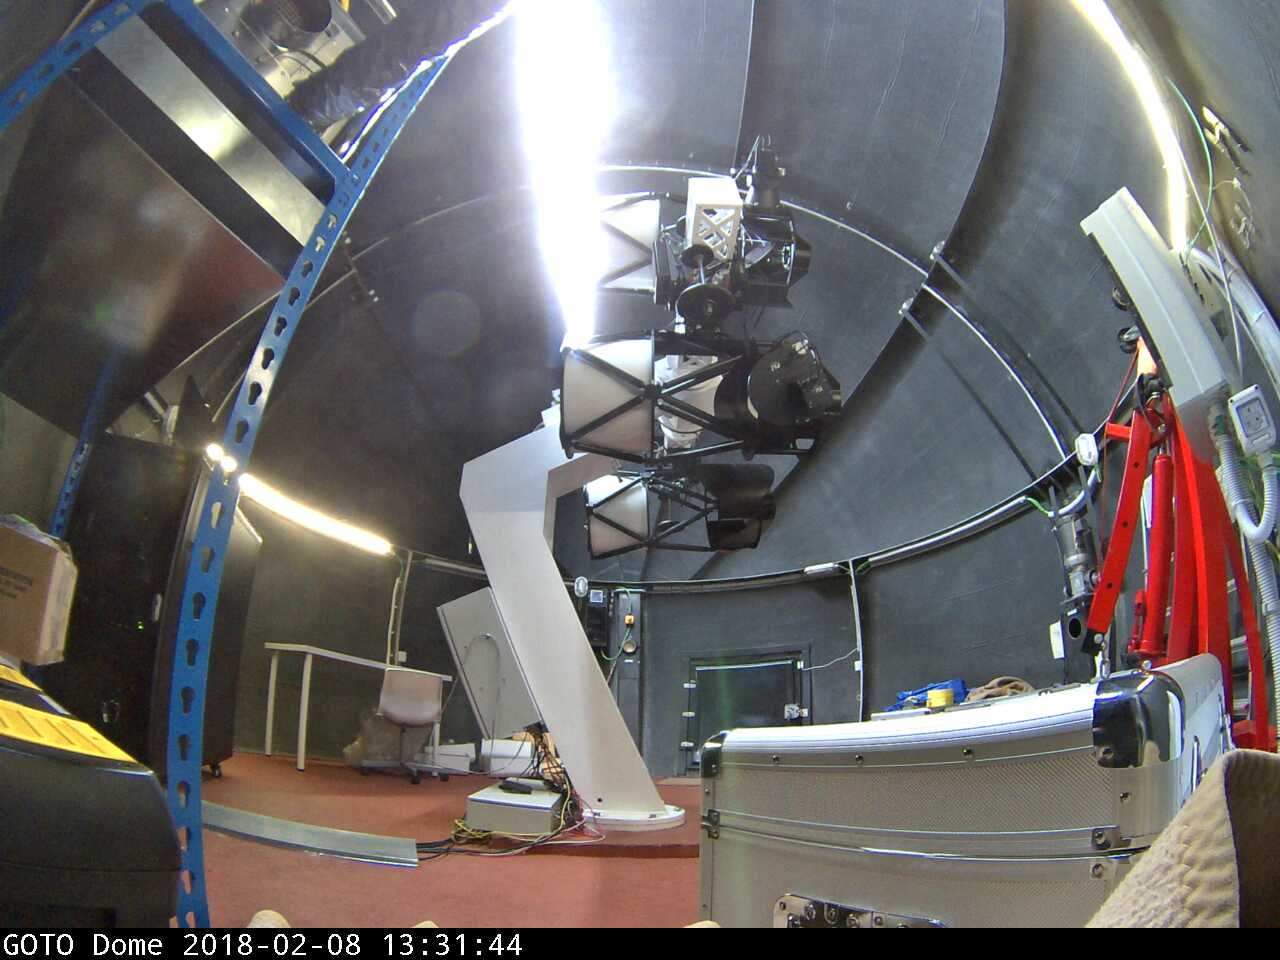
\includegraphics[width=0.45\textwidth]{images/ice_open.jpeg}
        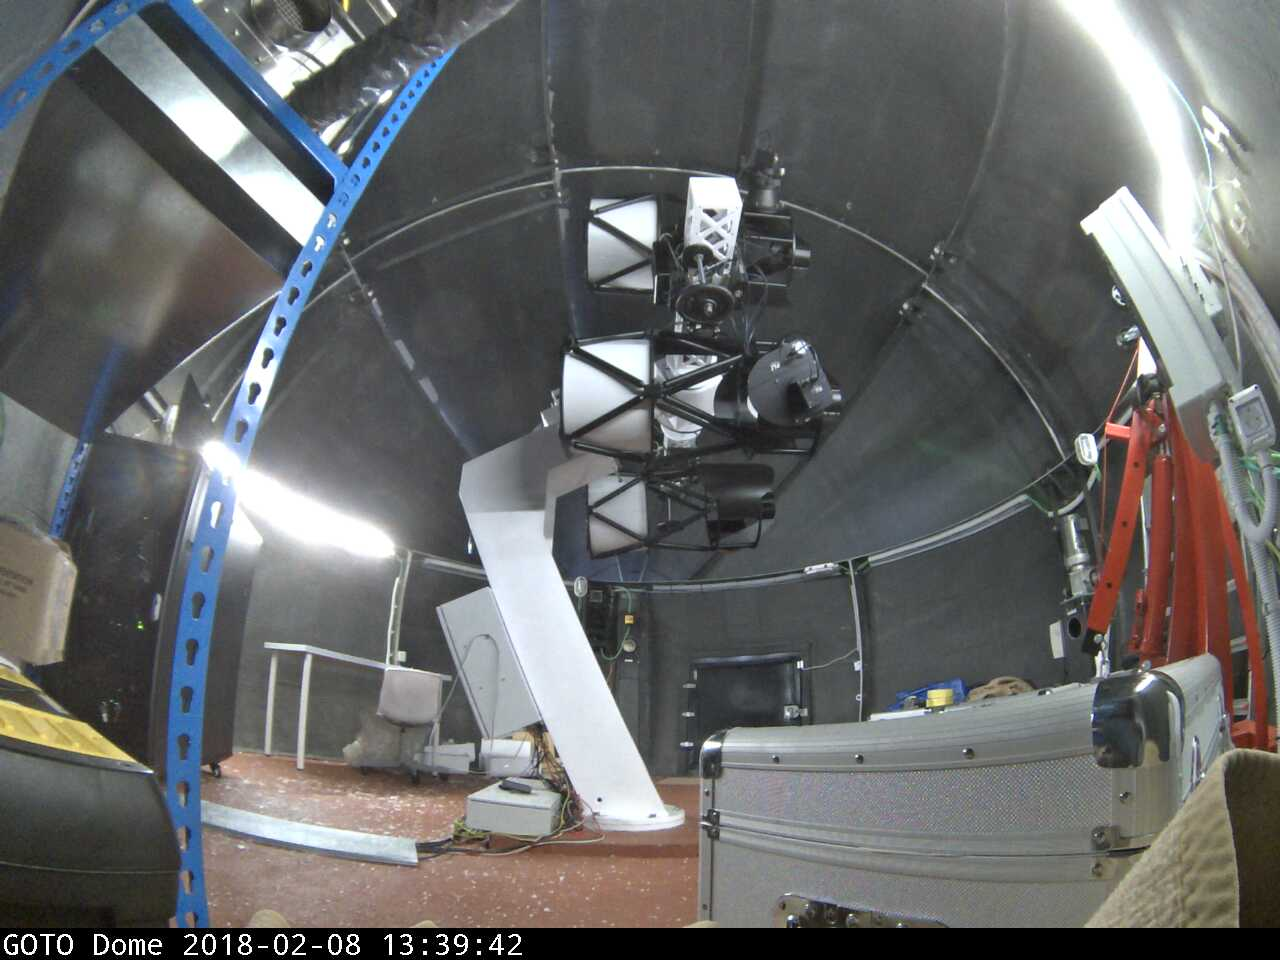
\includegraphics[width=0.45\textwidth]{images/ice_closed.jpeg}
    \end{center}
    \caption[Internal webcam images showing the dome open during a snowstorm]{
        Internal webcam images showing the dome open during the 2018 snowstorm.\\
        Left: The dome when the opening was discovered, with the upper shutter (which normally closes on the south side, to the left of the image) having been pulled past its limits by the weight of ice built up on the north side.\\
        Right: The dome after closing the shutter remotely. Moving the shutters caused a large amount of ice to dislodge and fall into the dome, thankfully missing the mirrors and camera hardware.
    }\label{fig:ice_internal}
\end{figure}

\begin{figure}[p]
    \begin{center}
    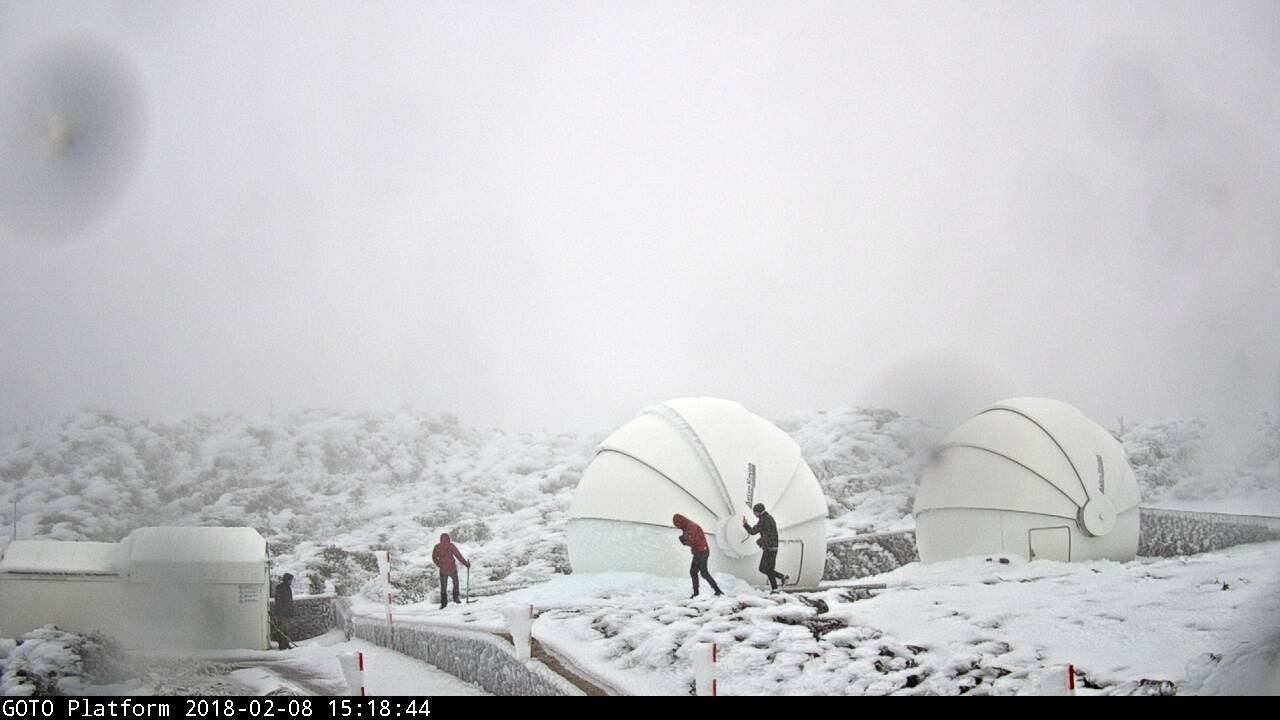
\includegraphics[width=0.88\textwidth]{images/ice_outside.jpeg}
    \end{center}
    \caption[External webcam image showing the ice rescue team]{
        External webcam image showing the ice rescue team. Note the build up of ice visible on the northern side of the upper shutter of the (empty) left-hand dome. A similar build up caused the upper shutter on the right-hand dome containing GOTO to be pulled open.
    }\label{fig:ice_external}
\end{figure}

\clearpage

\end{colsection}

% ~~~~~~~~~~~~~~~~~~~~

\end{colsection}

% ########################################
